\begin{evenBlock}{Foot Soldiers (10 min)}

\begin{minipage}[t]{\linewidth}
    \centering
    
    \begin{minipage}{.4\linewidth} % Left column and width
        \centering
        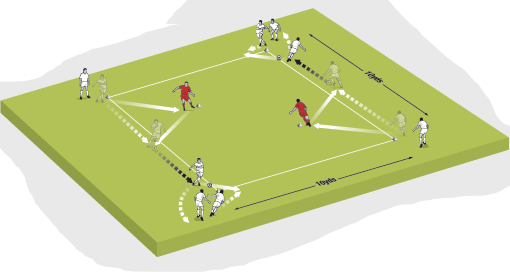
\includegraphics[width=\textwidth]{../img/Trimmed/FootSoldiers1}
        \vspace{6pt}
        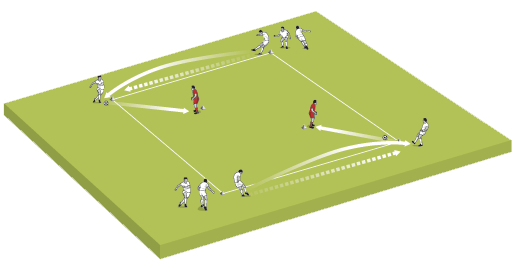
\includegraphics[width=\textwidth]{../img/Trimmed/Footsoldiers2}
    \end{minipage}
    \hspace{0.05\linewidth}
    \begin{minipage}{.5\linewidth} % Left column and width
        \textbf{Drill Description:}
        To use this simple warm-up mark out a 10x10-yard square with cones. Position a cone as shown for the central players. We have used 14 players in this activity, including two servers. You need balls and cones.
        \begin{enumerate}
        \setlength{\itemsep}{0pt}
        \setlength{\parskip}{0pt}
        \setlength{\parsep}{0pt}
        \item Place the two servers inside the square and arrange the remaining players around the four corners of the area use the central players to make one-two wall passes on opposite sides of the square and a first-time pass along the other sides of the square.
        \item Players should sidefoot their passes to the central players, who must make sure that they control the ball and pass it back to the running players so they don’t have to break their stride.
        \item You should swap the players over regularly, changing the two central wall passers. You must have two balls in play at once.
        \end{enumerate}

        \begin{enumerate}
        \setlength{\itemsep}{0pt}
        \setlength{\parskip}{0pt}
        \setlength{\parsep}{0pt}
        \item Play starts on both sides with a pass to the server who plays a one-two with the working player
        \item The player dribbles towards the cone and passes to the player at the cone
        \item The player at the next cone must be on the move to receive the ball and make a one touch pass to the next cone
        \item Players must follow the pass and keep moving around the square
        \item The receiving player for the one-two pass can take two touches because this needs to be an accurate move with a good weight on the pass
        \end{enumerate}

    \end{minipage}
\end{minipage}

\end{evenBlock}